W niniejszym rozdziale zostanie przedstawione oprogramowanie wykorzystane w pracy wraz z uzasadnieniem jego wyboru.

\section{Oprogramowanie do automatycznego testowania}

Na początku zostaną przedstawione najpopularniejsze narzędzia do automatyzacji testowania - JMeter oraz Selenium WebDriver. Zostanie też wspomniane o programie LoadRunner jako alternatywie dla pierwszego narzędzia.

\subsection{JMeter}

Popularnym narzędziem wykorzystywanym przede wszystkim do testów obciążeniowych aplikacji webowych jest \textbf{Apache JMeter}. Dzięki niemu można zarówno przeanalizować wydajność systemu lub serwisu, jak i pisać testy funkcjonalne. Stosuje wiele różnych typów serwerów i protokołów sieciowych czy komunikacyjnych (np. HTTP, HTTPS, SOAP, JDBS, LDAP, TCP, POP3). \cite{roman} oraz \cite{jmeter}. JMeter został zaimplementowany w języku Java, w związku z tym może on działać na różnych systemach operacyjnych.

\begin{figure}[H]
\centering
\captionsetup{justification=centering}

\includegraphics[width=0.8\textwidth]{Apache_JMeter.png}
\caption[Logo JMetera]{\label{fig:ham}Logo JMetera \\ źródło: \textit{https://commons.wikimedia.org/wiki/File:Apache$\_$JMeter.png}}
\end{figure}

Za pomocą JMetera można parametryzować testy, sprawdzać asercje (czy dany krok testowy zwraca to, czego oczekuje się w określonym teście) czy wprowadzać zmienne. Te właściwości będziemy wykorzystywać do pisania automatycznych testów funkcjonalnych właśnie w tym narzędziu.


JMeter składa się z następujących komponentów (na podstawie \cite{comp}):
\begin{itemize}
    \item \textit{Test Plan} - w nim znajdują się wszystkie komponenty i ustawienia;
    \item \textit{Samplers} - wykonują odpowiednie polecenia, które zwracają rezultaty z ich przebiegu (konkretnie, czy wykonał się prawidłowo, czas, rozmiar danych) za pomocą Listenerów;
    \item \textit{Config Elements} - ustawia domyślne wartości do późniejszego użycia przez kroki testowe;
    \item \textit{Listeners} - zbierają informacje o wykonaniu się kolejnych kroków dla testów, a także pozwalają zobaczyć czy zapisać rezultaty testów;
    \item \textit{Thread Groups} - określa pulę użytkowników, która wykona podane kroki testowe, czas przyspieszenia (czyli jak długo zajmie wystartowanie wszystkich wątków), ile razy wykonać test oraz czas startu i końca testu;
    \item \textit{(Logic) Controllers} - definiują, w jakim porządku mają się wykonać kroki testowe;
    \item \textit{Assertions} - sprawdzają, czy dany krok zwraca to, czego oczekujemy;
    \item \textit{Pre Processors} - wykonują polecenia przed wykonaniu kroku;
    \item \textit{Post Processors} - wykonują polecenia po wykonaniu kroku; 
    \item \textit{Timers} - liczniki wykonywane przed danym krokiem.
\end{itemize}

\begin{figure}[H]
\centering
\captionsetup{justification=centering}
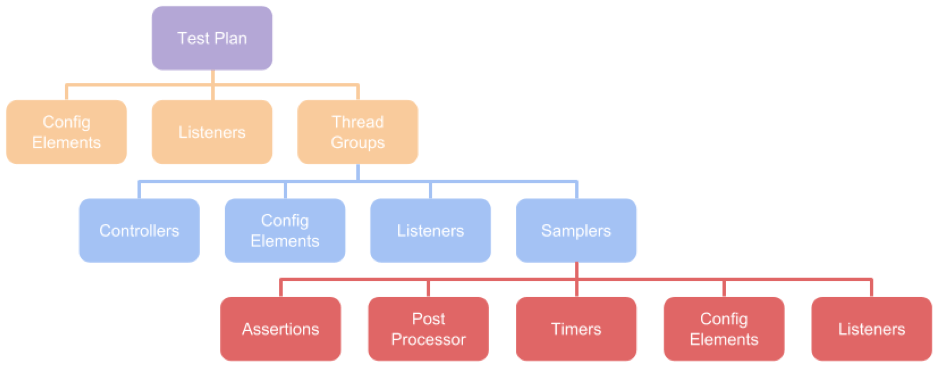
\includegraphics[width=1.05\textwidth]{jmeterComp.png}
\caption[Komponenty JMetera i zależności między nimi przedstawione w formie grafu]{\label{fig:ham}Komponenty JMetera i zależności między nimi przedstawione w formie grafu \\ źródło: https://cdn2.hubspot.net/hubfs/208250/Blog\_Images/jsel1.png}
\end{figure}


Szczegółowe informacje na temat JMetera można znaleźć na oficjalnej stronie: https://jmeter.apache.org/. 


\subsection{Load Runner}

Alternatywą dla JMetera jest \textit{Load Runner} - komercyjne narzędzie do przeprowadzania testów wydajnościowych za pomocą skryptów. Wykorzystuje się go również do testowania aplikacji desktopowych czy mobilnych. Podobnie jak JMeter, Load Runner może integrować się z róznymi IDE. \cite{lr}

\subsection{Selenium WebDriver} 
Bardzo często wykorzystywanym narzędziem do testowania automatycznego aplikacji webowych jest otwartoźródłowy \textit{Selenium WebDriver}. \cite{aut} Można w nim pisać skrypty testowe w różnych językach programowania, takich jak Java, Python, Ruby, Scala czy Perl. Tak jak wspomniany wcześniej JMeter, Selenium również wspiera mnóstwo systemów operacyjnych (Windows, Linux, Mac i inne), ale też  najpopularniejsze przeglądarki internetowe (Chrome, Firefox, Internet Explorer). \cite{selenium}


\begin{figure}[H]
\centering
\captionsetup{justification=centering}

\includegraphics[width=0.6\textwidth]{selenium.png}
\caption[Logo Selenium]{\label{fig:ham}Logo Selenium \\ źródło: \textit{https://www.trickydefects.com/wp-content/uploads/2018/02/selenium.png}}
\end{figure}

Dokładniejsze informacje o Selenium wraz z dokumentacją można znaleźć na oficjalnej stronie: https://www.seleniumhq.org/.

\begin{figure}[H]
\centering
\captionsetup{justification=centering}
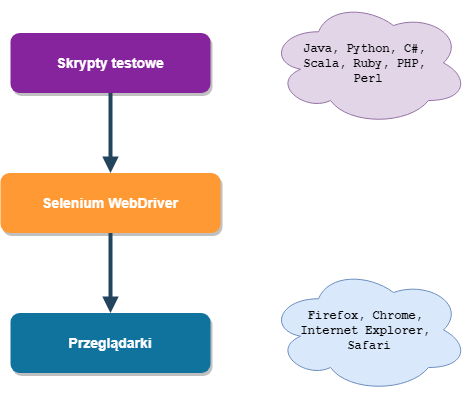
\includegraphics[width=0.9\textwidth]{SeleniumWorkflow.png}
\caption[Schemat działania Selenium WebDriver]{\label{fig:ham}Schemat działania Selenium WebDriver \\ źródło: opracowanie własne}
\end{figure}


\section{Platformy do pisania stron internetowych}
\subsection{WordPress}
Do napisania prostej aplikacji webowej, która zostanie poddana testowaniu, wykorzystano znaną platformę \textbf{WordPress} – darmowy i dostępny jako wolne oprogramowanie system zarządzania treścią (ang. \textit{Content Management System, CMS}), zaprojektowany przede wszystkim do obsługi blogów, oparty o język PHP oraz bazę danych MySQL. \cite{wpa}

\begin{figure}[H]
\centering
\captionsetup{justification=centering}

\includegraphics[width=0.8\textwidth]{WordPress_logo.png}
\caption[Logo WordPressa]{\label{fig:ham}Logo WordPressa \\ źródło: https://en.wikipedia.org/wiki/WordPress/media/File:WordPress\_logo.svg}
\end{figure}



WordPress jest używany przez ponad 60 milionów stron internetowych. Ponadto jest najbardziej popularnym CMS na świecie.\cite{succ} oraz \cite{wpa}

\subsection{Joomla!}

Drugą najpopularniejszą platformą CMS (\cite{stat}) jest \textbf{Joomla!} - również tak jak WordPress, darmowa i otwartoźródłowa. Została napisana w PHP i opiera się o bazę danych MySQL. \cite{joomla}


\section{BeanShell}

\textbf{BeanShell} jest językiem skryptowym, którego kompilator został napisany w Javie. Działa na platformie Java Virtual Machine (JVM). Wykorzystuje odmiany składni języka Java, a także polecenia skryptowe. JMeter stosuje ten język w swoim komponencie BeanShell Sampler do pisania skryptów. Można w tym komponencie importować biblioteki języka Java. \cite{beanshell}

\begin{figure}[H]
\centering
\captionsetup{justification=centering}
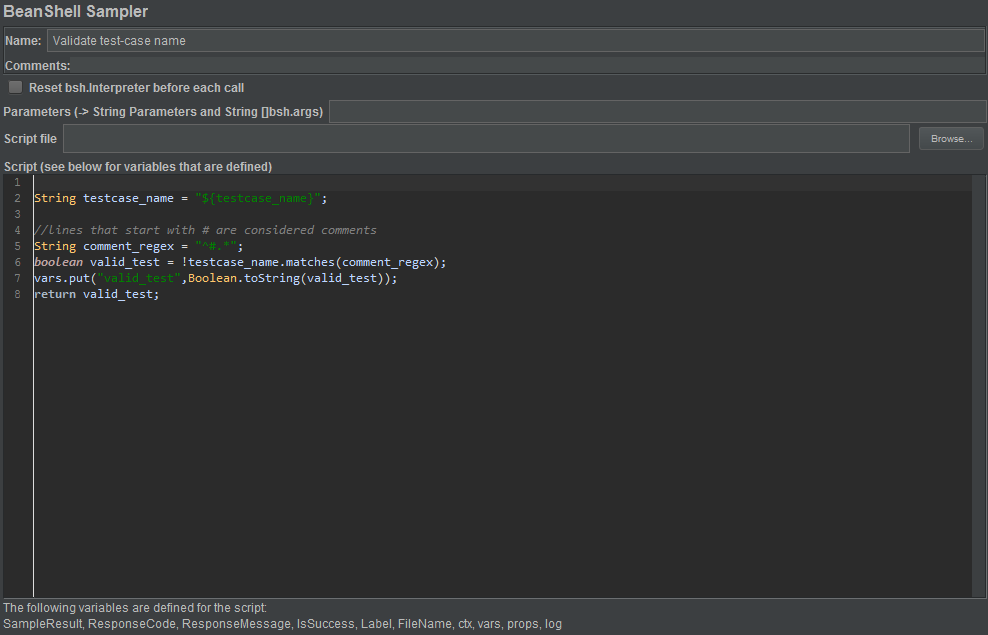
\includegraphics[width=1\textwidth]{BeanShell.PNG}
\caption[Przykład użycia BeanShell Samplera w JMeterze]{\label{fig:ham} Przykład użycia BeanShell Samplera w JMeterze \\ źródło: opracowanie własne}
\end{figure}




\section{Uzasadnienie wyboru JMetera oraz Selenium do przetestowania aplikacji internetowej}
Odpowiedni dobór narzędzi do automatyzacji testów jest niezwykle istotny, dlatego spośród wyżej wymienionych zostały wybrane dwa wyżej opisane: 
\begin{itemize}
    \item otwartoźródłowy JMeter ze względu na łatwą obsługę, szybkie wdrożenie, wparcie wielu protokołów (takich jak HTTP, JDBC czy LDAP) oraz możliwości przeprowadzenia w nim różnych rodzajów testów: od wydajnościowych, przez obciążeniowe, przeciążeniowe do nawet funkcjonalnych.
    \item Selenium WebDriver wykorzystywane w jmeterowym komponencie BeanShell Sampler ze względu na pisanie czytelnych skryptów do testowania aplikacji webowych.
\end{itemize}

Warto wspomnieć, że zarówno w JMeterze, jak i w Selenium można napisać automatyczne testy funkcjonalne do aplikacji internetowych. Oba te narzędzia są zaimplementowane w języku programowania Java, dzięki czemu można w nich pisać bez względu na system operacyjny. Zarówno JMeter, jak i Selenium WebDriver są oprogramowaniem, którego obsługi można się szybko nauczyć na podstawie szeroko dostępnych materiałów, kursów czy też dokumentacji. Oba te narzędzia cechują się szerokim wsparciem społeczności, dzięki czemu istnieje duża szansa, że zostało już znalezione rozwiązanie ewentualnych napotkanych problemów.

Jako alternatywa dla JMetera był rozważany LoadRunner, jednak dokonując porównania obu tych narzędzi, ostatecznie wybrano te pierwsze, co obrazuje poniższa tabela. 

\begin{table}[H]
\caption{Zestawienie cech JMetera z LoadRunnerem}
\label{my-label4}
\resizebox{\textwidth}{!}{%
\begin{tabular}{|
>{\columncolor[HTML]{C0C0C0}}l |c|c|}
\hline
\textbf{}                                                    & \multicolumn{1}{l|}{\cellcolor[HTML]{C0C0C0}\textbf{JMeter}} & \multicolumn{1}{l|}{\cellcolor[HTML]{C0C0C0}\textbf{Load Runner}} \\ \hline
\textbf{Wolne oprogramowanie}                                & \textbf{Tak}                                                   & \textbf{}                                                         \\ \hline
\textbf{Łatwość w obsłudze}                                  & \textbf{Tak}                                                   & \textbf{}                                                         \\ \hline
\textbf{Bogata dokumentacja}                                 & \textbf{Tak}                                                   & \textbf{Tak}                                                        \\ \hline
\textbf{Łatwość wdrożenia się}                               & \textbf{Tak}                                                   & \textbf{}                                                         \\ \hline
\textbf{Częste aktualizacje}                                 & \textbf{Tak}                                                   & \textbf{}                                                         \\ \hline
\textbf{Możliwość pisania testów funkcjonalnych}             & \textbf{Tak}                                                 & \textbf{Tak}                                                      \\ \hline
\textbf{Automatyzacja aplikacji webowych}                    & \textbf{Tak}                                                 & \textbf{Tak}                                                      \\ \hline
\textbf{Znajomość programowania}                             & \textbf{Niewymagana}                                         & \textbf{Tak}                                                        \\ \hline
\textbf{Łatwość pisania scenariuszy testowych}               & \textbf{Tak}                                                   & \textbf{}                                                         \\ \hline
\textbf{Wsparcie wielu protokołów}                           & \textbf{Tak}                                                   & \textbf{Tak}                                                        \\ \hline
\textbf{Możliwość obsługi na różnych systemach operacyjnych} & \textbf{Tak}                                                   & \textbf{Głównie Windows oraz Linux}                                 \\ \hline
\end{tabular}%
}
\end{table}

Decydującymi czynnikami wyboru JMetera zamiast LoadRunnera były: bezpłatne korzystanie, łatwa obsługa, szybkie wdrożenie się, prostota pisania scenariuszy testowych, możliwość pracy na wielu systemach operacyjnych czy wsparcie dużej ilości protokołów.

\section{Uzasadnienie wyboru WordPressa do napisania prostej aplikacji internetowej}

Spośród dwóch platform do pisania stron internetowych, mianowicie WordPress oraz Joomla!, wybrano tą pierwszą ze względu na łatwość obsługi i zerowy koszt utworzenia strony na potrzeby napisania prostych testów funkcjonalnych. 

\begin{table}[H]
\caption{Zestawienie zalet i wad dwóch najpopularniejszych platform CMS}
\label{my-label3}
\resizebox{\textwidth}{!}{%
\begin{tabular}{|
>{\columncolor[HTML]{C0C0C0}}l |l|l|}
\hline
\textbf{}       & \cellcolor[HTML]{C0C0C0}\textbf{WordPress}                                                                                                                                                                                                                                                     & \cellcolor[HTML]{C0C0C0}\textbf{Joomla!}                                                                                                                                                                                                                \\ \hline
\textbf{Zalety} & \begin{tabular}[c]{@{}l@{}}- Łatwa obsługa, zwłaszcza dla osób początkujących.\\ - Duża możliwość wyboru darmowych szablonów czy wtyczek.\\ - Nie jest wymagana znajomość programowania.\\ - Niski koszt utworzenia strony.\\ - Częste aktualizacje i łatwość ich zainstalowania.\end{tabular} & \begin{tabular}[c]{@{}l@{}}- Przy znajomości programowania można zbudować za jej \\ pomocą bardziej rozbudowane strony internetowe.\end{tabular}                                                                                                        \\ \hline
\textbf{Wady}   & - Słabsze możliwości serwera przy coraz większej liczbie wtyczek.                                                                                                                                                                                                                              & \begin{tabular}[c]{@{}l@{}}- Trudniejsza obsługa w porównaniu do WordPressa.\\ - Niska jakość szablonów.\\ - Mała liczba wtyczek (zarówno darmowych, jak i płatnych).\\ - Wysoki koszt utworzenia strony.\\ - Trudności przy aktualizacji.\end{tabular} \\ \hline
\end{tabular}%
}
\end{table}